\documentclass{article}
\usepackage[utf8]{inputenc}
\usepackage{hyperref}
\usepackage[left=20mm,top=20mm,right=20mm,bottom=20mm]{geometry}
\usepackage{etoolbox} %required for cover page
\usepackage{booktabs}
\usepackage[usestackEOL]{stackengine}
\usepackage[T1]{fontenc}
\usepackage[utf8]{inputenc}
\usepackage{bm}
\usepackage{graphicx}
\usepackage{subcaption}
\usepackage{amsmath}
\usepackage{amsfonts}
\usepackage{mathtools}
\usepackage{xcolor}
\usepackage{float}
\usepackage{hyperref}
\usepackage[capitalise]{cleveref}
\usepackage{enumitem,kantlipsum}
\usepackage{amssymb}
\usepackage[square,numbers,sort]{natbib}
\usepackage[ruled,vlined]{algorithm2e}
\usepackage{listings}
\usepackage{lscape}
\usepackage{longtable}
\usepackage{boldline}



\title{Laboratorio di Interazioni Fondamentali \\ Relazione esperienza 1}
\author{Irene Celestino}
\date{8/11/2022}

\begin{document}
\maketitle

\section{Introduzione e scopo dell'esperienza}
Lo scopo dell'esperienza preliminare è di usare per la prima volta i rivelatori di raggi cosmici, ovvero scintillatori e fotomoltiplicatori, e di stimare l'efficienza dei tre scintillatori, in particolare del secondo posto più in alto. 
\\
\\
I vari step dell'esperienza sono: 
\begin{itemize}
    \item [1.] studio del segnale in uscita dai 3 fotomoltiplicatori al variare della tensione di alimentazione
    \item [2.] utilizzo delle unità di discriminazione e di coincidenza, analisi del segnale in uscita e stima del ritardo da loro introdotto 
    \item [3.] conteggio del numero di eventi registrati per unità di tempo dai singoli fotomoltiplicatori e in coincidenza doppia o tripla
    \item [4.] stima dell'efficienza del secondo scintillatore come $$\epsilon_2 = \frac{n(1\&2\&3)}{n(1\&3)}$$
\end{itemize}

\subsection{Apparato sperimentale}
Gli strumenti utilizzati sono: 
\begin{itemize}
    \item 3 scintillatori plastici 
    \item 3 fotomoltiplicatori (9954B dell'azienda ET Enterprises) posti più in alto (indicati nella relazione come PM7, PM5 e PM4) 
    \item 1 unità di discriminazione a 4 ingressi
    \item 2 unità di coincidenza a 5 ingressi ciascuna
    \item 1 contatore a 7 ingressi con un segnale di clock interno
    \item il generatore di alta tensione e l'oscilloscopio digitale
\end{itemize}
L'apparato sperimentale è composto da 3 scintillatori plastici piani posti, di spessore di 2.5 cm e di forma data da un rettangolo di superficie 56 cm x 27 cm con poi una parte che va a stringersi sempre di più per arrivare al fotomoltiplicatore, lunga 30 cm.
Gli scintillatori sono orizzontali e posti parallelamente uno sopra l'altro e sono ricoperti da un materiale di plastica nero che scherma l'apparato dalla luce ambientale. \\
La distanza tra il primo e il secondo è di 16 cm, mentre quella tra il secondo e il terzo è di 7 cm. \\
A un'estremità di ogni scintillatore è collegato un fotomoltiplicatore, il cui segnale in uscita viene collegato al rack con un cavo coassiale nero di impedenza interna 50 Ohm e tempo di ritardo 6 ns.\\

\newpage
\section{Studio del segnale del primo fotomoltiplicatore (PM7)}
\subsection{Visualizzazione del segnale all'oscilloscopio}
Per prima cosa, ho collegato i vari cavi a setup spento: 
\begin{itemize}
    \item il fotomoltiplicatore è collegato al rack con un cavo coassiale nero con impedenza interna 50 Ohm e tempo di ritardo 6 ns
    \item dal rack ho collegato il segnale in uscita da PM7 al CH1 dell'oscilloscopio, con un cavo coassiale con tempo di ritardo 2 ns e terminando la linea con una resistenza da 50 Ohm per evitare riflessioni
    \item ho impostato l'oscilloscopio digitale con le scale di 25.0 ns/div, 20 mV/div e con il trigger con sorgente CH1, slope falling, soglia -40 mV, mode Normal
\end{itemize}
Ho poi acceso l'alimentatore di tensione partendo da una tensione di alimentazione di 1100 V. Fino a 1600 V non si ha una frequenza di trigger inferiore ai 10 Hz, mentre per le tensioni successive si hanno i risultati mostrati in tabella \ref{tabal}. \\
La frequenza di trigger cambia in continuazione, quindi ho riportato in tabella il range in cui si avevano la maggior parte dei valori, da cui si può vedere un andamento crescente all'aumentare dell'alimentazione. 

\begin{table}[h!]
\begin{center}
\begin{tabular}{|c|c|}
\hline
Tensione di alimentazione [kV] & Frequenza di trigger [Hz]\\
\hline
     1.600 & $<$ 10   \\
    1.700 & 10 $\div$ 30\\
    1.750  & 80 $\div$ 130\\
    1.770  & 120 $\div$ 200\\
    \hline
\end{tabular}
\end{center}
\caption{Andamento della frequenza di trigger al variare della tensione di alimentazione di PM7}\label{tabal}
\end{table}


Il segnale è composto da un picco verso il basso, della durata media di 10-20 ns, con un paio di picchettini alti in media 4-5 mV, che probabilmente sono dovuti alla riflessione nel cavo coassiale, in quanto né l'impedenza interna del cavo né la resistenza del tappo usato per terminare la linea sono esattamente 50 Ohm.\\
In figura \ref{f_PM} si può vedere il segnale generato dal fotomoltiplicatore PM7 alimentato a 1750 V.

\begin{figure}[h!]
\begin{center}
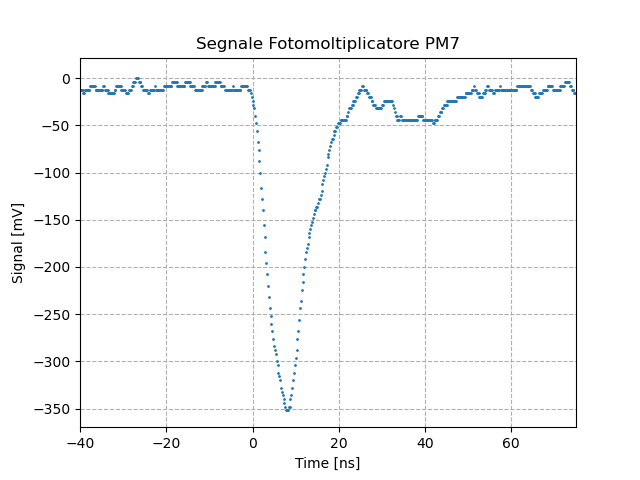
\includegraphics[scale=0.7]{Grafici/PM5_segnale.png}
\caption{Segnale generato da PM7 alimentato a 1750 V} \label{f_PM}
\end{center}
\end{figure}
\newpage

\subsection{Studio della frequenza di trigger al variare della soglia di trigger}
Visti i risultati della sezione precedente, ho deciso di settare l'alimentazione a 1750 V, in modo da avere una frequenza di trigger intorno ai 100 Hz quando la soglia è -40 mV. 
\\
Ho poi osservato come variava la frequenza di trigger modificando la soglia di trigger. Riporto in figura \ref{f1} l'andamento osservato della frequenza di trigger al variare della soglia. Come frequenza di trigger ho scelto per ogni valore della soglia un valore medio tra quelle riportate dall'oscilloscopio, ma le fluttuazioni di questo valore erano abbastanza ampie (circa il $30\%-40\%$ del valore medio). \\
In tabella \ref{tabfreq} ho riportato per ogni valore della tensione di soglia una media del valore minimo e del valore massimo tra cui oscillava la frequenza di trigger. \\ Come è ragionevole aspettarsi, più la soglia si abbassa meno è frequente osservare segnali. 


\begin{table}[h!]
    \centering
    \begin{tabular}{|c|c|c|c|}
        \hline
        Soglia [mV] & Frequenza di trigger minima [Hz]& Frequenza di trigger massima [Hz] & Frequenza di trigger media [Hz]\\
        \hline
            -60.0& 25& 44& 34\\
            -50.0& 30& 50& 40\\
            -40.0& 90& 120& 105 \\
            -30.0& 160& 240& 200\\
            -20.0& 290& 400& 345\\
            -15.0& 370& 530& 450\\
            -10.0& 750& 900& 825\\
        \hline
    \end{tabular}
    \caption{Frequenza di trigger al variare della tensione di soglia} \label{tabfreq}
\end{table}

\vspace{4mm}
\begin{figure}[h]
\begin{center}
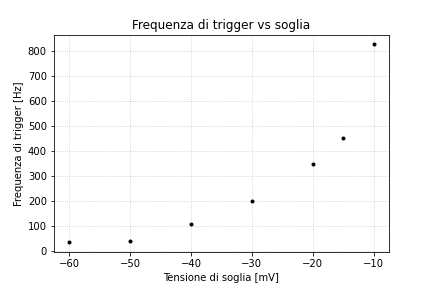
\includegraphics[scale=0.9]{Grafici/ftrigger_vs_soglia.png}
\caption{Stima della frequenza di trigger media al variare della soglia di trigger} \label{f1}
\end{center}
\end{figure}

\newpage

\subsection{Studio del segnale in uscita dal discriminatore}
Ho poi collegato il segnale in uscita da PM7 all'input di un canale del discriminatore ed ho visualizzato all'oscilloscopio sia il segnale di PM7 sia quello in uscita dal discriminatore. \\
Ho modificato le impostazioni del discriminatore, in modo da avere una soglia di -40 mV e un segnale della durata di circa 50 ns.\\
Con queste impostazioni, il segnale in uscita dal discriminatore è un segnale costante con il minimo a -1 V che si azzera di nuovo dopo circa 50 ns, come si può osservare in figura \ref{discr}.

\begin{figure}[h!]
\begin{center}
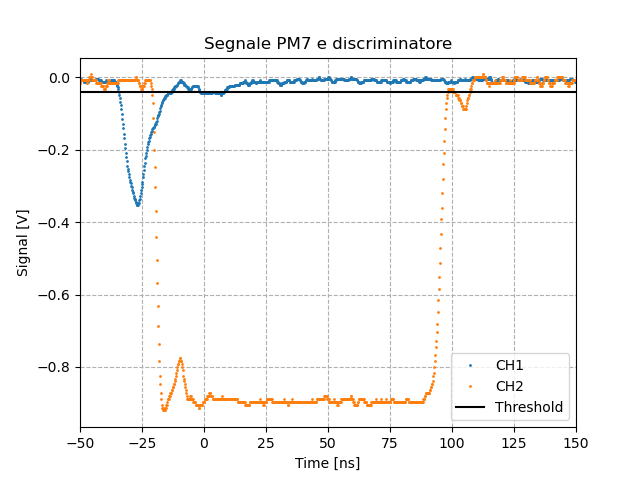
\includegraphics[scale=0.7]{Grafici/PM5_discriminatore.png}
\caption{Segnale generato da PM7 (CH1) e dal discriminatore (CH2) con soglia a -40 mV} \label{discr}
\end{center}
\end{figure}

\paragraph{Stima del ritardo introdotto dal discriminatore} A partire dalle forme d'onda osservate sull'oscilloscopio ho stimato il ritardo introdotto dal discriminatore rispetto al segnale del fotomoltiplicatore.\\
Cavi usati per i collegamenti:
\begin{itemize}
    \item Collegamento PM7-input del discriminatore: cavo con ritardo di 2 ns
    \item Collegamento input del discriminatore - CH1 dell'oscilloscopio: cavo con ritardo di 2 ns
     \item Collegamento output del discriminatore - CH2 dell'oscilloscopio: cavo con ritardo di 4 ns
\end{itemize}
Con questi cavi il ritardo che si osserva sull'oscilloscopio tra il segnale del fotomoltiplicatore e quello del discriminatore è proprio il ritardo introdotto dal discriminatore. 
\\
Infatti il segnale di PM7 impiega un tempo di 2ns+2ns = 4ns per arrivare sull'oscilloscopio attraverso i due cavi, mentre quello in uscita dal discriminatore 4ns attraverso il cavo più lungo.
\\
\\
Ho misurato con i cursori dell'oscilloscopio i due tempi a cui il segnale del fotomoltiplicatore e del discriminatore sono a circa metà della loro discesa. In particolare, per un singolo segnale ho misurato le quantità riportate in tabella \ref{tab1}.

\newpage
\begin{table}[h!]
    \centering
    \begin{tabular}{|c|c|c|}
        \hline
        Canale & Minimo del segnale & Istante di tempo a cui il segnale è a metà\\
        \hline
            CH1 & -79.2 mV & -2.00 ns \\
            CH2 & -1.06 V & 14.2 ns   \\
        \hline
    \end{tabular}
    \caption{Dati per la stima del ritardo introdotto dal discriminatore} \label{tab1}
\end{table}
Da questa misura si ricava che il ritardo introdotto dal solo discriminatore è di 16.2 ns. \\Se invece vogliamo considerare anche il ritardo introdotto dai cavi rispetto al momento in cui il segnale parte dal rack, bisogna aggiungere 4 ns.

\subsection{Contatore NIM in singola}
Ho collegato il segnale in uscita dal discriminatore a un ingresso del contatore NIM, in modo da contare il numero di eventi per unità di tempo e confrontare questo risultato con la frequenza di trigger dell'oscilloscopio. \\
\\Impostazioni del discriminatore e del contatore: 
\begin{itemize}
    \item Soglia del discriminatore: -40 mV
    \item Durata del conteggio: 10000 cicli di clock, cioè 10 s
\end{itemize}
\paragraph{Terminazione del cavo che collega l'uscita del discriminatore all'ingresso del contatore}
Dato che la resistenza in ingresso del contatore è di 50 Ohm, si può collegare direttamente l'uscita del discriminatore all'ingresso del contatore senza terminare con una resistenza da 50 Ohm. 
\\Ho provato ad aggiungere comunque una T con un tappo da 50 Ohm e i conteggi sono circa raddoppiati. Questo effetto è dovuto alle riflessioni del segnale nel cavo coassiale se non trova in uscita la stessa impedenza interna del cavo. 
\\
Ho notato però un fenomeno curioso: se aggiungo un tappo da 50 Ohm i conteggi raddoppiano solo in alcuni ingressi del contatore NIM, mentre in altri il numero di eventi per unità di tempo è circa lo stesso con e senza la resistenza aggiuntiva.
\\
In ogni caso, tutte le misure descritte da qui in avanti sono state prese senza aggiungere il tappo da 50 Ohm all'ingresso del contatore NIM.
\subsubsection{Confronto tra i conteggi e la frequenza di trigger} Idealmente, impostando la stessa soglia per il discriminatore e per il trigger dell'oscilloscopio, la frequenza di trigger e il numero di conteggi al secondo dovrebbero essere uguali, o almeno dello stesso ordine di grandezza. \\
Ho quindi provato ad impostare per entrambi una soglia di -40 mV ed ho misurato un numero di conteggi in 10 s pari a 1623. Il numero di conteggi al secondo era 162.3 s$^{-1}$, mentre la frequenza di trigger media era tra i 30 e i 40 Hz. \\
\\
Una possibile spiegazione di questa discordanza può essere il fatto che la soglia dell'oscilloscopio in realtà è diversa da -40 mV. \\Ho infatti cambiato manualmente la soglia dell'oscilloscopio fino ad arrivare alla situazione in cui a volte il segnale del discriminatore era spento mentre quello del fotomoltiplicatore era visualizzato all'oscilloscopio, ovvero fino a una tensione di soglia per il trigger di -21.6 mV. \\ Questa nuova soglia per il trigger è più alta della soglia effettiva che fa scattare il discriminatore: il segnale del discriminatore è nullo quando il segnale del fotomoltiplicatore è sotto la soglia di trigger ma sopra la soglia del discriminatore. \\Se però si sceglie la tensione di soglia per cui gli eventi in cui il discriminatore è nullo sono pochi, allora la soglia di trigger è abbastanza vicina a quella del discriminatore.\\
Infatti, con la soglia di trigger impostata a -21.6 mV la frequenza di trigger è in media 140-150 Hz, molto più vicina ai 162.3 conteggi al secondo misurati con il contatore.
\\
Ho quindi deciso di lasciare la soglia dell'oscilloscopio a -21.6 mV.
\newpage
\subsubsection{Numero di conteggi per unità di tempo al variare della tensione di alimentazione del fotomoltiplicatore}

Ho poi cambiato la tensione di alimentazione del fotomoltiplicatore e ogni volta attivato il contatore per 10 s, in modo da vedere come cambia il numero di conteggi al secondo con la tensione di alimentazione. \\
\\
In figura \ref{f2} ho riportato il grafico del numero di conteggi al secondo al variare della tensione di alimentazione in un range tra 1600 e 1975 V. \\
Da notare che la scala verticale è logaritimica, perché il numero di conteggi al secondo aumenta molto velocemente. 

\begin{figure}[h]
\begin{center}
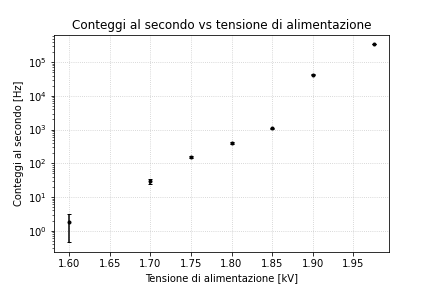
\includegraphics[scale=0.9]{Grafici/conteggi_vs_alimentazione.png}
\caption{Andamento del numero di conteggi al secondo al variare della tensione di alimentazione del fotomoltiplicatore PM7} \label{f2}
\end{center}
\end{figure}


\section{Studio dei tre fotomoltiplicatori più in alto (PM7, PM5 e PM4)}
Ho ripetuto alcune misure descritte nella parte precedente anche per i due fotomoltiplicatori posti sotto a PM7, ovvero PM5 e PM4. \\
In particolare, per prima cosa ho collegato i fotomoltiplicatori al discriminatore e al contatore, in modo da trovare la tensione di alimentazione per cui il numero di conteggi  per unità di tempo era intorno ai 100 cps.
\\
Come impostazioni sui due canali del discriminatore per PM5 e PM7 ho usato le stesse per PM7, ovvero tensione di soglia a -40 mV e durata del segnale discriminato di circa 50 ns. 
\\
\\
Per avere un numero di conteggi per unità di tempo costante pari a circa 100 cps bisogna alimentare in modo diverso i tre fotomoltiplicatori. In tabella \ref{tab2} ho riportato le tensioni di alimentazione per cui si hanno circa 100 conteggi per secondo per ognuno dei tre fotomoltiplicatori. 
\begin{table}[h!]
    \centering
    \begin{tabular}{|c|c|c|}
        \hline
        Fotomoltiplicatore & Tensione di alimentazione & Conteggi per secondo\\
        \hline
            PM7 & 1740 V& 98 cps   \\
            PM5 &  1685 V& 125 cps  \\
            PM4 & 1670 V& 90 cps \\
        \hline
    \end{tabular}
    \caption{Tensioni di alimentazione e conteggi in singola per i tre fotomoltiplicatori}
    \label{tab2}
\end{table}

\newpage
\section{Unità di coincidenza}
Nel rack sono presenti due unità di coincidenza, ognuna con cinque ingressi e due tipi di uscita, LIN e OUT. \\
La prima (figura \ref{LIN}) è un segnale che è diverso da zero per l'intervallo temporale in cui tutti gli ingressi attivati sono contemporaneamente accesi ed è ampio circa 8 V, mentre la seconda (figura \ref{OUT}) è un breve impulso di durata 10 ns e di ampiezza di 8 V che si attiva quando l'unità rileva una coincidenza tra i segnali in ingresso. 

\begin{figure}[h!]
\begin{center}
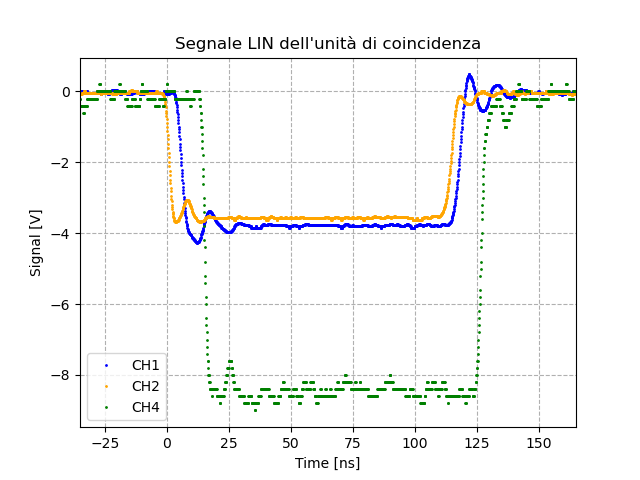
\includegraphics[scale=0.6]{Grafici/LIN_segnale.png}
\caption{Uscita LIN dell'unità di coincidenza (CH4) tra il segnale discriminato di PM7 (CH1) e di PM5 (CH2). Per ragioni puramente grafiche ho moltiplicato in figura il segnale dei due discriminatori per 4, in modo da distinguere bene le due forme d'onda (la loro ampiezza infatti è di circa 1 V in realtà).} \label{LIN}
\end{center}
\end{figure}


\begin{figure}[h!]
\begin{center}
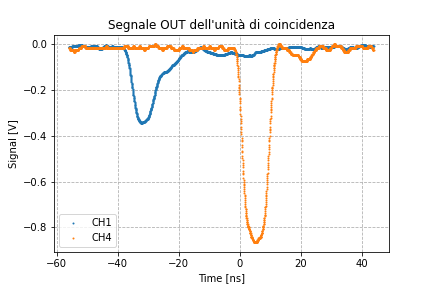
\includegraphics[scale=0.6]{Grafici/OUT_segnale.png}
\caption{Uscita OUT dell'unità di coincidenza (CH4) tra il segnale discriminato di PM7 e di PM5. In CH1 è rappresentato il segnale del fotomoltiplicatore PM5 (moltiplicato per 10 per ragioni grafiche), scelta fatta per confrontare il segnale OUT con un segnale di durata temporale analoga. \\Da notare che il ritardo tra CH1 e CH4 (di circa 40 ns) è dovuto sia al discriminatore sia all'unità di coincidenza, oltre al fatto che probabilmente il segnale in PM7 è scattato qualche ns dopo PM5.} \label{OUT}
\end{center}
\end{figure}


\newpage 
\subsection{Ritardo introdotto dall'unità di coincidenza}
Per prima cosa, ho studiato le coincidenze tra i primi due fotomoltiplicatori (PM7 e PM5), collegando i rispettivi segnali discriminati a due ingressi di un'unità di coincidenza.\\
Ho visualizzato all'oscilloscopio i due segnali discriminati di PM7 e di PM5 e l'uscita LIN dell'unità di coincidenza, in modo da stimare il ritardo introdotto dall'unità di coincidenza. 
\\
\\
Cavi usati per i collegamenti: 
\begin{itemize}
    \item Collegamento uscita discriminatori-ingresso coincidenza: cavi con ritardo di 2 ns
    \item Collegamento uscita discriminatori-oscilloscopio: cavi con ritardo di 2 ns
     \item Collegamento uscita LIN dell'unità di coincidenza-oscilloscopio: 4ns
\end{itemize}
In questo modo, il ritardo che si osserva all'oscilloscopio tra i segnali discriminati e il segnale in uscita dall'unità di coincidenza è proprio quello introdotto da quest'ultima. 
\\
Ho quindi misurato con i cursori dell'oscilloscopio gli istanti di tempo in cui i segnali discriminati dei due fotomoltiplicatori (visualizzati in CH1 e CH2) e il segnale in uscita dall'unità di coincidenza (visualizzato in CH4) sono scesi a metà della loro ampiezza, ottenendo i seguenti risultati: 

\begin{table}[h!]
    \centering
    \begin{tabular}{|c|c|c|}
        \hline
        Canale & Minimo del segnale & Istante di tempo a cui il segnale è a metà\\
        \hline
            CH1 (PM7 discriminato) & -992 mV & 6 ns \\
            CH2 (PM5 discriminato)& -912 mV& 0.7 ns   \\
            CH4 (uscita LIN unità di coincidenza) & -8.40 V & 15 ns\\
        \hline
    \end{tabular}
    \caption{Dati per la stima del ritardo introdotto dall'unità di coincidenza}
    \label{tab3}
\end{table}
A partire da queste misure ho stimato il ritardo introdotto dall'unità di coincidenza come la differenza tra il tempo in cui è scattato il primo fotomoltiplicatore (6 ns) e il tempo in cui è scattata l'unità di coincidenza, ottenendo un ritardo di 9 ns.
\\
In figura \ref{LINrit} si può vedere uno zoom della figura \ref{LIN} nella fase di discesa dei tre segnali, in modo da visualizzare graficamente il ritardo, stimato come la differenza temporale tra la discesa di CH1 (il fotomoltiplicatore che scatta dopo) e quella di CH4. 
\begin{figure}[h!]
\begin{center}
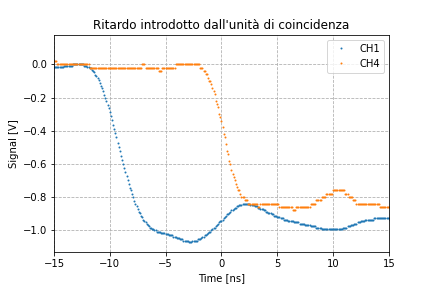
\includegraphics[scale=0.65]{Grafici/LIN_ritardo.png}
\caption{Uscita LIN dell'unità di coincidenza (CH4) tra il segnale discriminato di PM7 (CH1) e di PM5 (CH2). Per ragioni puramente grafiche ho moltiplicato in figura il segnale dei due discriminatori per 4, in modo da distinguere bene le due forme d'onda (la loro ampiezza infatti è di circa 1 V in realtà).} \label{LINrit}
\end{center}
\end{figure}

\subsection{Conteggi e incertezze sui conteggi}
Le misure di efficienza si basano sui conteggi dei segnali in uscita dai discriminatori e dalle unità di coincidenza, quindi per prima cosa ho stimato l'incertezza nella misura dei conteggi. 
\\
La statistica dei conteggi per unità di tempo è una poissoniana, quindi potrebbe risultare ragionevole prendere come incertezza la radice quadrata del valore misurato, in quanto per le poissoniane la varianza è uguale alla media. 
\\
Tuttavia, ho ripetuto molte volte la misura dei conteggi per unità di tempo in singola e in doppia tenendo fisse le alimentazioni dei fotomoltiplicatori e ho notato che il range in cui variano le misure è inferiore alla radice del numero di conteggi. \\
A titolo di esempio, riporto in tabella \ref{errcont} diverse misure dei conteggi in singola (acquisite in un intervallo di 100 s) del fotomoltiplicatore PM7 alimentato sempre a 1740 V. 

\begin{table}[h!]
\centering
\begin{tabular}{|c|c|}
\hline
Conteggi per secondo cps & $\sigma =\sqrt{\text{cps}}$ \\ 
 \hline
\hline 
96.72 &  9.83 \\ 
\hline 
98.52 &  9.93 \\ 
\hline 
94.57 &  9.72 \\ 
\hline 
97.07 &  9.85 \\ 
\hline 
94.16 &  9.70 \\ 
\hline 
95.76 &  9.79 \\ 
\hline 
99.49 &  9.97 \\ 
\hline 
97.47 &  9.87 \\ 
\hline 
99.45 &  9.97 \\ 
\hline 
97.00 &  9.85 \\ 
\hline 
94.84 &  9.74 \\ 
\hline 
96.15 &  9.81 \\ 
\hline 
92.03 &  9.59 \\ 
\hline 
96.48 &  9.82 \\ 
\hline 
96.02 &  9.80 \\ 
\hline 
96.16 &  9.81 \\ 
\hline 
94.67 &  9.73 \\ 
\hline 
92.38 &  9.61 \\ 
\hline 
\end{tabular}
\caption{Fluttuazioni della misura dei conteggi per secondo in singola per PM7}\label{errcont}
\end{table}

Il valore medio dei conteggi per secondo è 96.05, con una media delle radici dei conteggi di 9.80. \\
Invece, l'errore massimo di queste misure, cioè $\frac{\text{max(cps) - min(cps)}}{2}$, è 3.73, inferiore all'errore stimato con la radice del numero di conteggi. Ancora di più è basso lo scarto quadratico medio, pari a 2.02.
\\
Per il fotomoltiplicatore PM4 (alimentato a 1670 V) si ottengono risultati analoghi: la media dei cps è 92.49, la media delle radici è 9.62, mentre l'errore massimo è 5.33 e lo scarto quadratico medio è 3.03.
\\
Dato però che per la maggior parte dei conteggi ho preso una sola misura una volta fissata l'alimentazione, considererò sempre come errore la radice del numero di conteggi per secondo, anche se questo valore può essere una sovrastima dell'intervallo in cui possono variare le misure dei conteggi. 
\newpage
\subsection{Conteggi delle coincidenze doppie, triple e dell'efficienza}

Per questa prima parte ho lavorato fissando le alimentazioni dei tre fotomoltiplicatori in modo da avere un rate di conteggi in singola di circa 100 cps, come indicato in sezione 3. In particolare, le alimentazioni soni 1740 V per PM7, 1685 V per PM5 e 1670 V per PM4.
\\
Ho poi misurato i conteggi delle coincidenze in doppia per ogni coppia di fotomoltiplicatorei e in tripla, ottenendo i risultati riportati in tabella \ref{tabdoppie}. Nell'ultima colonna è presente una prima stima dell'efficienza, calcolata come rapporto tra numero di coincidenze triple e numero di coincidenze doppie degli altri due fotomoltiplicatori.

\begin{table}[h!]
\centering
\begin{tabular}{|c|c|c|c|c|}
\hline
Fotomoltiplicatore &  Singola [cps] &  Coincidenza doppia [cps] & Coincidenza tripla [cps]  & Efficienza \\ 
\hline
\hline 
PM7 & $98.5 \pm 9.9$ & & &\\ 
PM5  & $123.9 \pm 11.1$ & $1\&3=7.37 \pm 2.71$  & $7.09 \pm 2.66$ & $\epsilon_2= 0.96 \pm 0.36$ \\ 
PM4  & $94.1 \pm 9.7$ & & &\\ 
\hline 
PM7 &  $100.1 \pm 10.0$ & & &\\ 
PM5  & $126.3 \pm 11.2$ & $1\&2 = 11.80 \pm 3.44$  & $7.90 \pm 2.81$ & $\epsilon_3= 0.67 \pm 0.23$\\ 
PM4 & $88.1 \pm 9.4$ & &  &\\ 
\hline 
PM7  & $94.2 \pm 9.7$ & & &\\ 
PM5  & $126.3 \pm 11.2$ & $2\& 3 = 14.98 \pm 3.87$  & $6.23 \pm 2.50$ & $\epsilon_1= 0.42 \pm 0.17$\\ 
PM4  & $87.0 \pm 9.3$ & & & \\ 
\hline
\end{tabular}
\caption{Conteggi in coincidenza doppia e tripla ad alimentazioni fissate}\label{tabdoppie}
\end{table}

\section{Efficienza dei fotomoltiplicatori al variare dell'alimentazione}

\subsection{Efficienza del secondo fotomoltiplicatore (PM5) al variare della sua alimentazione}
Per prima cosa, ho studiato l'andamento dell'efficienza del secondo fotomoltiplicatore (PM5) variando solo la sua tensione di alimentazione e tenendo fisse le altre due, a 1740 V per PM7 e 1670 V per PM4.
\\
L'efficienza di PM5 può essere stimata come $\epsilon_2 = \frac{n(1\&2\&3)}{n(1\&3)}$. \\ 
Per quanto riguarda le incertezze, dato che prendevo contemporaneamente le misure di $n(1\&2\&3)$ e di $n(1\&3)$, ho considerato i conteggi in doppia senza errore, in quanto ogni volta ridefiniscono il $100\%$ dei conteggi e non importa quanto il loro valore fluttui. 
Per questo motivo, ho considerato solo l'incertezza su $n(1\&2\&3)$, prendendo la radice del numero dei conteggi. \\
La misura dell'efficienza è data quindi in prima battuta, senza considerare le coincidenze accidentali, da: 
\begin{equation}
\epsilon_2 = \frac{n(1\&2\&3)}{n(1\&3)} \pm  \frac{\sqrt{n(1\&2\&3)}}{n(1\&3)}
\end{equation}

\subsubsection{Tabella con le misure per $\epsilon_2$}
Ho variato la tensione di alimentazione del secondo fotomoltiplicatore tra 1500 V e 1900 V e per ogni valore ho misurato per 100 s il numero di conteggi in singola dei tre fotomoltiplicatori, in coincidenza doppia $1\&3$ e in coincidenza tripla $1\&2\&3$.
\\
In tabella \ref{tabepsilon2} si possono vedere tutte le misure che ho preso con le relative incertezze. 
\\
Tutte le misure dell'efficienza di PM5 sono state riportate in figura \ref{fepsilon2}. 
\newpage

\begin{table}[H]
\centering
\begin{tabular}{|c|c|c|c|c|c|}
\hline
Fotomoltiplicatore & Alimentazione PM5 & Conteggi in singola [cps] & $1 \& 3$  [cps]&  $1\&2\& 3$ [cps]& $\epsilon_2$\\ 
 \hline
\hline 
PM7 & & $92.0 \pm 9.6$ & & & \\ 
PM5 & 1500 & $7.0 \pm 2.6$& $7.5 \pm 2.7$  & $1.7 \pm 1.3$ & $0.23 \pm 0.17$\\ 
PM4 & & $89.6 \pm 9.5$ & & & \\ 
\hline 
PM7 & & $96.0 \pm 9.8$ & & & \\ 
PM5 & 1520 & $9.6 \pm 3.1$& $6.7 \pm 2.6$  & $2.4 \pm 1.5$ & $0.36 \pm 0.23$\\ 
PM4 & & $89.8 \pm 9.5$ & & & \\ 
\hline 
PM7 & & $96.2 \pm 9.8$ & & & \\ 
PM5 & 1540 & $13.7 \pm 3.7$& $6.8 \pm 2.6$  & $3.4 \pm 1.8$ & $0.49 \pm 0.27$\\ 
PM4 & & $88.8 \pm 9.4$ & & & \\ 
\hline 
PM7 & & $94.8 \pm 9.7$ & & & \\ 
PM5 & 1550 & $16.3 \pm 4.0$& $6.4 \pm 2.5$  & $3.6 \pm 1.9$ & $0.57 \pm 0.30$\\ 
PM4 & & $91.4 \pm 9.6$ & & & \\ 
\hline 
PM7 & & $96.2 \pm 9.8$ & & & \\ 
PM5 & 1575 & $26.6 \pm 5.2$& $6.8 \pm 2.6$  & $4.9 \pm 2.2$ & $0.72 \pm 0.33$\\ 
PM4 & & $90.8 \pm 9.5$ & & & \\ 
\hline 
PM7 & & $97.0 \pm 9.8$ & & & \\ 
PM5 & 1600 & $39.9 \pm 6.3$& $7.1 \pm 2.7$  & $6.2 \pm 2.5$ & $0.88 \pm 0.35$\\ 
PM4 & & $92.4 \pm 9.6$ & & & \\ 
\hline 
PM7 & & $92.4 \pm 9.6$ & & & \\ 
PM5 & 1625 & $58.1 \pm 7.6$& $7.1 \pm 2.7$  & $6.6 \pm 2.6$ & $0.93 \pm 0.36$\\ 
PM4 & & $88.9 \pm 9.4$ & & & \\ 
\hline 
PM7 & & $94.7 \pm 9.7$ & & & \\ 
PM5 & 1650 & $82.1 \pm 9.1$& $6.8 \pm 2.6$  & $6.6 \pm 2.6$ & $0.96 \pm 0.37$\\ 
PM4 & & $89.0 \pm 9.4$ & & & \\ 
\hline 
PM7 & & $98.5 \pm 9.9$ & & & \\ 
PM5 & 1685 & $123.9 \pm 11.1$& $7.4 \pm 2.7$  & $7.1 \pm 2.7$ & $0.96 \pm 0.36$\\ 
PM4 & & $98.1 \pm 9.9$ & & & \\ 
\hline 
PM7 & & $94.6 \pm 9.7$ & & & \\ 
PM5 & 1695 & $140.4 \pm 11.8$& $7.2 \pm 2.7$  & $7.0 \pm 2.6$ & $0.97 \pm 0.37$\\ 
PM4 & & $94.6 \pm 9.7$ & & & \\ 
\hline 
PM7 & & $97.1 \pm 9.9$ & & & \\ 
PM5 & 1710 & $163.5 \pm 12.8$& $7.1 \pm 2.7$  & $6.9 \pm 2.6$ & $0.97 \pm 0.37$\\ 
PM4 & & $94.2 \pm 9.7$ & & & \\ 
\hline 
PM7 & & $95.8 \pm 9.8$ & & & \\ 
PM5 & 1730 & $204.7 \pm 14.3$& $6.9 \pm 2.6$  & $6.8 \pm 2.6$ & $0.99 \pm 0.38$\\ 
PM4 & & $93.9 \pm 9.7$ & & & \\ 
\hline 
PM7 & & $96.7 \pm 9.8$ & & & \\ 
PM5 & 1750 & $244.4 \pm 15.6$& $6.7 \pm 2.6$  & $6.7 \pm 2.6$ & $0.99 \pm 0.38$\\ 
PM4 & & $99.5 \pm 10.0$ & & & \\ 
\hline 
PM7 & & $94.2 \pm 9.7$ & & & \\ 
PM5 & 1780 & $368.0 \pm 19.2$& $7.0 \pm 2.6$  & $6.9 \pm 2.6$ & $0.98 \pm 0.37$\\ 
PM4 & & $93.7 \pm 9.7$ & & & \\ 
\hline 
PM7 & & $99.5 \pm 10.0$ & & & \\ 
PM5 & 1810 & $710.8 \pm 26.7$& $7.4 \pm 2.7$  & $7.3 \pm 2.7$ & $0.99 \pm 0.37$\\ 
PM4 & & $95.8 \pm 9.8$ & & & \\ 
\hline 
PM7 & & $97.5 \pm 9.9$ & & & \\ 
PM5 & 1850 & $1311.1 \pm 36.2$& $7.2 \pm 2.7$  & $7.2 \pm 2.7$ & $0.99 \pm 0.37$\\ 
PM4 & & $92.6 \pm 9.6$ & & & \\ 
\hline 
PM7 & & $99.5 \pm 10.0$ & & & \\ 
PM5 & 1870 & $1551.7 \pm 39.4$& $6.9 \pm 2.6$  & $6.8 \pm 2.6$ & $0.99 \pm 0.38$\\ 
PM4 & & $91.5 \pm 9.6$ & & & \\ 
\hline 
PM7 & & $96.5 \pm 9.8$ & & & \\ 
PM5 & 1900 & $1858.2 \pm 43.1$& $7.2 \pm 2.7$  & $7.1 \pm 2.7$ & $0.99 \pm 0.37$\\ 
PM4 & & $90.4 \pm 9.5$ & & & \\ 
\hline
\end{tabular}
\caption{Conteggi per la stima di $\epsilon_2$}\label{tabepsilon2}
\end{table}

\newpage

\subsubsection{Grafico di $\epsilon_2$ al variare dell'alimentazione di PM5}
In figura \ref{fepsilon2} sono riportate le misure dell'efficienza di PM5 al variare della sua alimentazione. 
\\
Si può vedere che la sua efficienza è molto alta (intorno al $98-99\%$) nel regime in cui è pienamente funzionante, ovvero oltre i 1600 V, mentre scendendo sotto questa tensione l'efficienza cala velocemente. \\
In particolare, la tensione di alimentazione per cui l'efficienza è dimezzata è 1540 V.

\begin{figure}[h!]
\begin{center}
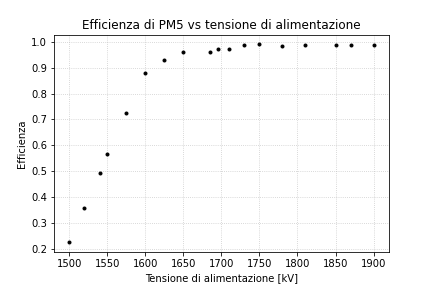
\includegraphics[scale=0.7]{Grafici/epsilon_vs_alimentazione_PM5.png}
\caption{Efficienza $\epsilon_2$ al variare della tensione di alimentazione del secondo fotomoltiplicatore PM5, mantenendo le altre due alimentazioni costanti} \label{fepsilon2}
\end{center}
\end{figure}

\subsubsection{Coincidenze accidentali}

Il numero di coincidenze doppie accidentali tra il primo e il terzo fotomoltiplicatore può essere stimato nel seguente modo. \\
Definiamo le seguenti quantità: 
\begin{itemize}
\item $R_1$ = numero di conteggi per secondo del primo fotomoltiplicatore
\item $R_3$ = numero di conteggi per secondo del terzo fotomoltiplicatore
\item $w_i$ = durata temporale del segnale in uscita dal discriminatore che va in ingresso all'unità di coincidenza (nel nostro caso vale 50 ns per entrambi i fotomoltiplicatori)
\item $w_{\text{min}}$ = tempo minimo per cui si devono sovrapporre due segnali in ingresso all'unità di coincidenza per avere in uscita un segnale diverso da zero (nel nostro caso vale circa 2 ns)
\item $\Delta t$ = durata dell'acquisizione
\end{itemize}
Una stima del numero di coincidenze accidentali è data da: 
\begin{equation}
\label{eq_accidental}
n(1\&3)_{\text{acc}} = \Delta t \cdot R_1 \cdot R_3 \cdot (w_1+w_3-2w_{\text{min}}) \simeq 0.085
\end{equation}
Quindi il numero medio di coincidenze accidentali, 0.085, è molto minore rispetto al numero delle coincidenze doppie $1\&3$ misurate (in media circa 7), e si possono trascurare in questo caso le coincidenze accidentali. 
\newpage
\subsubsection{Nota sui conteggi in singola di PM5 a tensioni di alimentazione alte}

Si può vedere in tabella \ref{tabepsilon2} che per i valori più alti di tensione di alimentazione il numero di conteggi in singola di PM5 cresce in modo abbastanza veloce e questo effetto può sembrare in prima battuta dovuto al fatto che il fotomoltiplicatore lavora a pieno regime. 
\\
Ho notato tuttavia sull'oscilloscopio, mentre osservavo il segnale di PM5 e del suo discriminatore, che il segnale di PM5 a queste alimentazioni è molto rumoroso. 
In particolare, anche quando il segnale dovrebbe essere a 0 V in realtà presenta delle fluttuazioni che in certi casi riescono a superare i 40 mV di ampiezza. \\
Il discriminatore, però, è settato su una soglia di -40 mV e quindi può scattare anche a causa delle fluttuazioni, determinando un numero di conteggi maggiore rispetto al numero di eventi effettivamente registrati dal fotomoltiplicatore. 
\\
\\
Una soluzione a questo inconveniente potrebbe essere alzare la soglia del discriminatore se si vuole lavorare a tensioni di alimentazione alte.\\
Tuttavia, il fatto che i conteggi in singola siano falsati non influenza in nessun modo la misura di efficienza, perché le unità di coincidenza scattano solo se ci sono più discriminatori attivati contemporaneamente ed è abbastanza raro che PM4 e PM7 scattino nello stesso istante in cui il discriminatore di PM5 scatta a causa di una fluttuazione. 
\\
\\
In ogni caso, ho acquisito con l'oscilloscopio i segnali di PM5 e del discriminatore quando quest'ultimo è scattato a causa di una fluttuazione più ampia di -40 mV (figura \ref{fnoise}). \\
In figura, si vede che le fluttuazioni subito dopo il picco principale mantengono il segnale del discriminatore a -800 mV per più di 50 ns, perché l'unità di discriminazione vede più volte un segnale che scende sotto soglia. Inoltre, a 200 ns CH1 mostra un'altra fluttuazione appena sotto i -40 mV che fa scattare nuovamente il discriminatore. \\
Quest'ultima fluttuazione potrebbe anche essere dovuta a riflessioni nel cavo coassiale perché anche se è stato terminato tutto con resistenze da 50 Ohm ci può essere un piccolo discostamento di questa resistenza dal valore nominale e se il segnale del fotomoltiplicatore è ampio le riflessioni possono superare i -40 mV.

\begin{figure}[h!]
\begin{center}
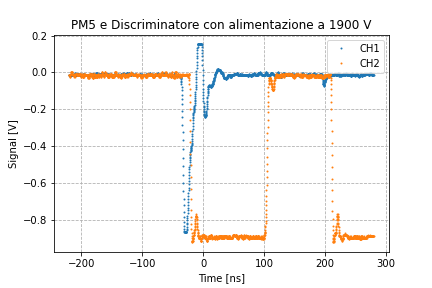
\includegraphics[scale=0.7]{Grafici/PM5_rumore.png}
\caption{In CH1 c'è il segnale di PM5, alimentato a 1900 V, mentre in CH2 il segnale in uscita dal discriminatore, che scatta una seconda volta a causa di una fluttuazione. Il segnale di CH2 è stato traslato verso l'alto di 100 mV per ragioni grafiche, in modo da far vedere meglio la fluttuazione di CH1 a un tempo di circa 200 ns} \label{fnoise}
\end{center}
\end{figure}

\newpage
\subsection{Efficienza del primo fotomoltiplicatore (PM7) al variare della sua alimentazione}
Analogamente, poi ho studiato l'andamento dell'efficienza del primo fotomoltiplicatore (PM7) variando solo la sua tensione di alimentazione e tenendo fisse le altre due, a 1685 V per PM5 e 1670 V per PM4.
\\
In tabella \ref{tabepsilon1} e in figura  \ref{fepsilon1}  si possono vedere le misure di efficienza, intesa come rapporto tra coincidenze triple e doppie, per il primo fotomoltiplicatore. L'andamento che si osserva è analogo a PM5, ma il valore massimo di $\epsilon_1$ è molto più basso, pari al $58\%$.\\
Questo si può spiegare con il fatto che, mentre se una particella che passa per il primo e il terzo scintillatore deve aver attraversato necessariamente il secondo, possono esserci benissimo particelle con traiettorie che intersecano solo il primo scintillatore. 

\begin{table}[H]
\centering
\begin{tabular}{|c|c|c|c|c|c|}
\hline
Fotomoltiplicatore & Alimentazione PM7 & Conteggi in singola [cps] & $2 \& 3$  [cps]&  $1\&2\& 3$ [cps]& $\epsilon_1$\\ 
 \hline
\hline 
PM7 & & $6.7 \pm 2.6$ &  & &\\ 
PM5 & 1670 & $125.0 \pm 11.2$ & $14.8 \pm 3.8$  & $1.7 \pm 1.3$ & $0.11 \pm 0.09$\\ 
PM4 & & $88.4 \pm 9.4$ &  & &\\ 
\hline 
PM7 & & $94.2 \pm 9.7$ &  & &\\ 
PM5 & 1740 & $126.3 \pm 11.2$ & $15.0 \pm 3.9$  & $6.2 \pm 2.5$ & $0.42 \pm 0.17$\\ 
PM4 & & $87.0 \pm 9.3$ &  & &\\ 
\hline 
PM7 & & $1039.0 \pm 32.2$ &  & &\\ 
PM5 & 1800 & $118.9 \pm 10.9$ & $14.4 \pm 3.8$  & $8.3 \pm 2.9$ & $0.58 \pm 0.20$\\ 
PM4 & & $81.8 \pm 9.0$ &  & &\\ 
\hline 
PM7 & & $800.5 \pm 28.3$ &  & &\\ 
PM5 & 1850 & $125.5 \pm 11.2$ & $14.5 \pm 3.8$  & $7.9 \pm 2.8$ & $0.54 \pm 0.19$\\ 
PM4 & & $87.1 \pm 9.3$ &  & &\\ 
\hline 
PM7 & & $27723.3 \pm 166.5$ &  & &\\ 
PM5 & 1900 & $124.2 \pm 11.1$ & $14.9 \pm 3.9$  & $7.7 \pm 2.8$ & $0.52 \pm 0.19$\\ 
PM4 & & $89.4 \pm 9.5$ &  & &\\ 
\hline
\end{tabular}
\caption{Conteggi per la stima di $\epsilon_1$}\label{tabepsilon1}
\end{table}

\begin{figure}[h!]
\begin{center}
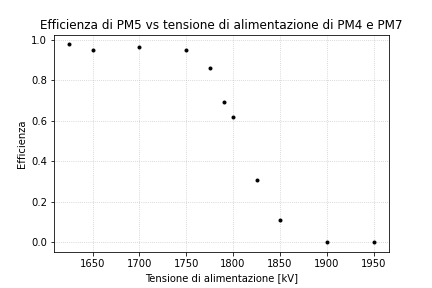
\includegraphics[scale=0.7]{Grafici/epsilon_vs_alimentazione_PM7.png}
\caption{Efficienza $\epsilon_1$ al variare della tensione di alimentazione del secondo fotomoltiplicatore PM7, mantenendo le altre due alimentazioni costanti} \label{fepsilon1}
\end{center}
\end{figure}

\newpage
\subsection{Efficienza del terzo fotomoltiplicatore (PM4) al variare della sua alimentazione}
Infine ho studiato l'andamento dell'efficienza del terzo fotomoltiplicatore (PM4) variando solo la sua tensione di alimentazione e tenendo fisse le altre due, a 1685 V per PM5 e 1740 V per PM7.
\\
In tabella \ref{tabepsilon3} e in figura  \ref{fepsilon3} (nella prossima pagina) si possono vedere le misure di efficienza, intesa come rapporto tra coincidenze triple e doppie, per il terzo fotomoltiplicatore. 

\begin{table}[H]
\centering
\begin{tabular}{|c|c|c|c|c|c|}
\hline
Fotomoltiplicatore & Alimentazione PM4 & Conteggi in singola [cps] & $1 \& 2$  [cps]&  $1\&2\& 3$ [cps]& $\epsilon_3$\\ 
\hline
\hline 
PM7 & & $95.3 \pm 9.8$ &  & & \\ 
PM5 & 1550 & $126.1 \pm 11.2$ & $11.2 \pm 3.4$  & $0.5 \pm 0.7$& $0.04 \pm 0.06$\\ 
PM4 & & $2.3 \pm 1.5$ &  & &\\ 
\hline 
PM7 & & $96.5 \pm 9.8$ &  & & \\ 
PM5 & 1600 & $125.3 \pm 11.2$ & $11.7 \pm 3.4$  & $2.9 \pm 1.7$& $0.25 \pm 0.15$\\ 
PM4 & & $10.7 \pm 3.3$ &  & &\\ 
\hline 
PM7 & & $94.4 \pm 9.7$ &  & & \\ 
PM5 & 1640 & $127.1 \pm 11.3$ & $11.4 \pm 3.4$  & $5.6 \pm 2.4$& $0.49 \pm 0.21$\\ 
PM4 & & $37.3 \pm 6.1$ &  & &\\ 
\hline 
PM7 & & $100.1 \pm 10.0$ &  & & \\ 
PM5 & 1670 & $126.3 \pm 11.2$ & $11.8 \pm 3.4$  & $7.9 \pm 2.8$& $0.67 \pm 0.24$\\ 
PM4 & & $88.1 \pm 9.4$ &  & &\\ 
\hline 
PM7 & & $95.1 \pm 9.8$ &  & & \\ 
PM5 & 1700 & $125.7 \pm 11.2$ & $10.6 \pm 3.3$  & $7.4 \pm 2.7$& $0.70 \pm 0.26$\\ 
PM4 & & $166.5 \pm 12.9$ &  & &\\ 
\hline 
PM7 & & $99.3 \pm 10.0$ &  & & \\ 
PM5 & 1710 & $127.1 \pm 11.3$ & $9.3 \pm 3.0$  & $6.6 \pm 2.6$& $0.71 \pm 0.28$\\ 
PM4 & & $171.5 \pm 13.1$ &  & &\\ 
\hline 
PM7 & & $98.0 \pm 9.9$ &  & & \\ 
PM5 & 1750 & $126.9 \pm 11.3$ & $11.2 \pm 3.3$  & $8.3 \pm 2.9$& $0.74 \pm 0.26$\\ 
PM4 & & $828.5 \pm 28.8$ &  & &\\ 
\hline 
PM7 & & $94.8 \pm 9.7$ &  & & \\ 
PM5 & 1850 & $124.9 \pm 11.2$ & $10.4 \pm 3.2$  & $8.0 \pm 2.8$& $0.77 \pm 0.27$\\ 
PM4 & & $192482.3 \pm 438.7$ &  & &\\ 
\hline 
PM7 & & $95.7 \pm 9.8$ &  & & \\ 
PM5 & 1900 & $126.4 \pm 11.2$ & $11.6 \pm 3.4$  & $8.7 \pm 3.0$& $0.76 \pm 0.26$\\ 
PM4 & & $244425.2 \pm 494.4$ &  & &\\ 
\hline
\end{tabular}
\caption{Conteggi per la stima di $\epsilon_3$}\label{tabepsilon3}
\end{table}

\begin{figure}[h!]
\begin{center}
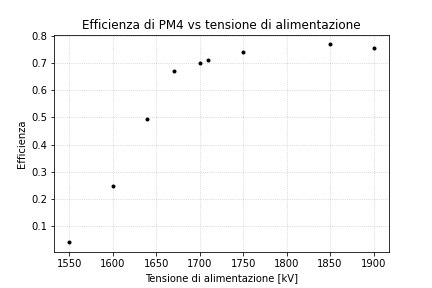
\includegraphics[scale=0.7]{Grafici/epsilon_vs_alimentazione_PM4.png}
\caption{Efficienza $\epsilon_3$ al variare della tensione di alimentazione del terzo fotomoltiplicatore PM4, mantenendo le altre due alimentazioni costanti} \label{fepsilon2}
\end{center}
\end{figure}
\subsubsection{Commenti sulle misure di efficienza dei tre fotomoltiplicatori}
L'andamento che si osserva per PM4 è analogo a PM5 e PM7, anche se il valore massimo di $\epsilon_3$, pari al $77\%$,è molto più basso rispetto a $\epsilon_2$, ma più alto di $\epsilon_1$.\\
Per lo stesso motivo descritto nella sezione precedente ci aspettiamo che $\epsilon_3 < \epsilon_2$. Però, vedendo com'è fatto l'apparato sperimentale, possiamo anche intuire perché $\epsilon_3 > \epsilon_1$. \\
Infatti, la distanza tra il primo e il secondo fotomoltiplicatore è di 16 cm, mentre quella tra il secondo e il terzo è di 7 cm. Quindi le particelle che attraversano solo il primo sono di più di quelle che attraversano solo il terzo perché il primo è più lontano ed anche più in alto. \\
Tra tutte e tre le stime $\epsilon_1$, $\epsilon_2$ e $\epsilon_3$, solo la seconda ha il significato fisico di efficienza di uno scintillatore, perché è estremamente raro trovare un raggio cosmico che passa solo da PM5, cosa che non si può dire per gli atri due.



\end{document}